\documentclass[dvipsnames]{beamer}


\usepackage[utf8]{inputenc}
\usepackage[T1]{fontenc}

\usepackage{lmodern} % get rid of fontsize warning
\usepackage{tikz}
%\usetikzlibrary{calc,chains,shapes,positioning}
\usepackage{pgfplots}
\pgfplotsset{compat=1.18}
\usepackage{verbatim}
\usepackage{amsmath}
\usepackage{textpos}
\usepackage{gradient-text}
% \usepackage[dvipsnames]{xcolor}
\usepackage{graphicx}
\usepackage[normalem]{ulem}
%\usepackage[colorlinks=false,pdfborder={0 0 0}]{hyperref}



\title{git - the stupid content tracker}
\subtitle{git eats trees.}
\author{Henry S. {Grasshorn Gebhardt}}
%\institute[The Pennsylvania State University]
%{Department of Astronomy and Astrophysics}
%\date{February 26, 2013}



\newcommand{\comp}[1]{{\tt #1}}


\begin{document}

\frame{\titlepage}

\section[Outline]{}
\frame{
    \frametitle{Outline}
    \tableofcontents
}


\section{Introduction to Version Control}
\frame{
    \frametitle{Version Control? Version Control.}
    % Premise: Code is text.

    % \bigskip
    Version control helps to:
    \begin{itemize}
        \item Save history.
        \item Keep track of changes.
        \item Merge code.
        \item Share code. (Don't be a git!)
        \item Consistency checking, e.g., when running code or configs elsewhere.
        \item \ldots
    \end{itemize}

    Git, Mercurial, \sout{Bazaar}, \sout{SVN (why bother?)}, \sout{CVS},
    \sout{Monotone}, \sout{DARCS}, \ldots

    ``Theory of Patches''
}

\frame{
    \frametitle{Git was created by Linus Torvalds for Linux kernel development}

    Linux developers used to use \texttt{BitKeeper} until it wasn't free anymore.

    \smallskip

    So Linus Torvalds created git, which always had a reputation for being too
    complicated to use. First release 7 April 2005.

    \smallskip

    There are {\color{red}\emph{plumbing}} commands and
    {\color{blue}\emph{porcelain}} commands.

    \smallskip

    \centering
    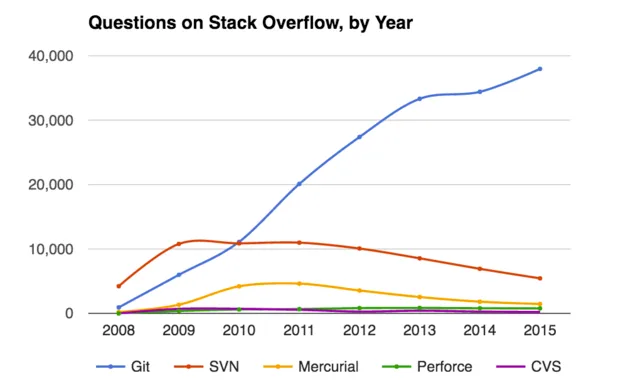
\includegraphics[width=0.7\textwidth]{./git-so}
}


\frame{
    \frametitle{What is a patch?}

    Patches are text files that show \gradientRGB{cha}{10,10,255}{100,255,10}\gradientRGB{nges}{100,255,10}{255,10,10}.

    \bigskip

    {\color{Green} Create a patch:}\\
    \texttt{\$ diff -Naur file1 file2 > changes.patch}
    \medskip

    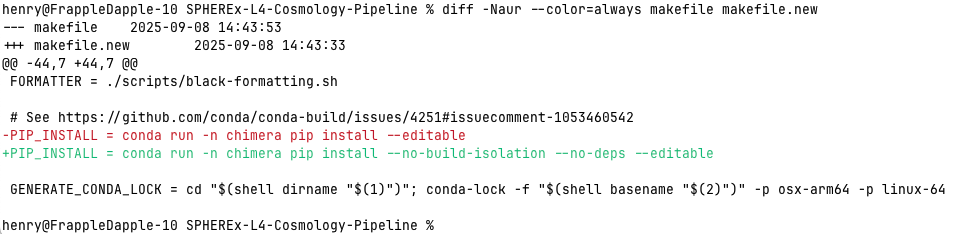
\includegraphics[width=\textwidth]{create_patch.png}

    \bigskip

    {\color{blue} Apply a patch:}\\
    \texttt{\$ patch -p1 < changes.patch}
}


\section{Theory}
\frame{
    \frametitle{Git History}

    \begin{center}
        \url{https://git-scm.com}
    \end{center}
    \bigskip

    History is a DAG (directed acyclic graph). \emph{Explain graph.}
    \bigskip

    Distributed, not centralized. \emph{Every clone has the full history.}
}

\frame{
    \frametitle{Git doesn't know about directories\ldots whaaat?}

    Git only knows content. (blobs)
    \bigskip

    And how that content is assembled. (trees)
    \bigskip

    And history. (commits)
    \bigskip

    Each commit stores the full source code (no patches!).
}


\frame{
    \frametitle{blobs, trees, and commits are identified by their SHA1-sum}

    A hash is a (hopefully) unique number to identify some information, like a
    file.
    \medskip

    SHA-1 is a 160-bit number. It happens to be cryptographically secure.
    \medskip

    Blobs, trees, and commits are identified by their SHA1 sum.
    \medskip

    $\Rightarrow$ Efficient de-duplication and compression
}


\frame{
    \frametitle{Terminology: blah, blah, blah,\ldots}
    WORKDIR \\
    GITDIR \\
    HEAD \\
    Index \\
    Local repository \\
    Upstream repository \\
    Stash
}


\section{git commands}
\frame{
    \frametitle{git cheat sheet}

    Here's the \emph{porcelain}:
    \bigskip

    %\url{https://services.github.com/kit/downloads/github-git-cheat-sheet.pdf}
    \url{https://about.gitlab.com/images/press/git-cheat-sheet.pdf}
    \vfill
    Initialization once per machine ({\tt \char`~/.gitconfig}):
    \begin{quote}
        \tt
        \$ git config -$\,$-global user.name "Henry VIII" \\
        \$ git config -$\,$-global user.email "h@here.com"
    \end{quote}
}


\frame{
    \frametitle{Initial checkout}
    Existing repository:
    {\tt\\
        \hspace{0.3cm}\$ git clone ssh://git@git.psu.edu/hsg113/test.git
    }
    \vfill
    New repository:
    {\tt\\
        \hspace{1cm}\$ mkdir newrepo \\
        \hspace{1cm}\$ cd newrepo \\
        \hspace{1cm}\$ git init
    }
}


\frame{
    \frametitle{Directory structure}
    {\tt
        \hspace{1cm}newrepo/ \\
        \hspace{1.5cm}    .git/ \\
        \hspace{1.5cm}    README.md \\
        \hspace{1.5cm}    doc/ \\
        \hspace{1.5cm}    src/ \\
        \hspace{1.5cm}    test/ \\
    }
}


\frame{
    \frametitle{git help command}

    Useful commands:

    \begin{description}[Other]
        \item[git status] Where am I?
        \item[git diff] What did I just do?
        \item[git diff -$\,$-staged] What will I do?
        \item[git log] What have I done?
        \item[gitk -$\,$-all] Let's climb trees!
        \item[git describe -$\,$-always -$\,$-tags] Who am I?
    \end{description}
}

\frame{
    \frametitle{Trees, yum!}
    \framesubtitle{git eats trees\ldots nom,nom}

    Branches are cheap!

    \begin{description}
        \item[git branch <name>] Let's make a new branch.
        \item[git branch -d] Never mind.
        \item[git checkout <name>] Let's climb over to that branch.
        \item[git checkout -b <newname> <starthere>] Checkout and make a new branch.
        \item[git merge <otherbranches>...] Trees eating trees!
        \item[git rebase -i <branchname>] Clean up your history!
    \end{description}
}


\frame{
    \frametitle{Pushing and pulling}
    \color{red} Put graph of distributed computing.

    {\tt
        \hspace{1cm}\$ git push <remote> <localbranch>:<remotebranch> \\
        \hspace{1cm}\$ git push -$\,$-set-upstream \\
        \hspace{1cm}\$ git pull \\
        \hspace{1cm}\$ git remote -v \\
    }
}


\frame{
    \frametitle{Workflow}
}


\frame{
    \frametitle{Play nice together!}
    \begin{center}
        {\tt \$ git svn}
        \vfill
        Works by calling ``{\tt git fast-import}''.
    \end{center}
}


\frame{
    \frametitle{Hosting your git repository}
    Companies:
    \begin{itemize}
        \itemindent3em
        \item[Github:] \url{github.com}
        \item[Gitlab:] \url{gitlab.com}
        \item[\ldots]
    \end{itemize}
    \bigskip
    Your own:
    \begin{itemize}
        \itemindent3em
        \item[SSH server:] Your own workstation/server.
        \item[SSH server:] \url{http://gitolite.com/} (probably overkill)
        \item[\ldots]
    \end{itemize}
    \bigskip
    {\tt
        \hspace{1cm}\$ mkdir -p \char`~/repos/newawesomeproject.git\\
        \hspace{1cm}\$ cd \char`~/repos/newawesomeproject.git\\
        \hspace{1cm}\$ git init -$\,$-bare
    }
}


\frame{
    \frametitle{Ah, I did something stupid\ldots}

    Recovery might be possible by looking into {\tt .git/logs/}.

    \bigskip
    {\tt git reflog} parses it for you.
}


\frame{
    \frametitle{Other commands}

    Graphs: {\tt git log -$\,$-graph}
    \bigskip

    More graphs: {\tt gitk -$\,$-all}
    \bigskip

    Tags: {\tt git tag}
    \bigskip

    Hooks: {\tt man githooks}; {\tt cd .git/hooks/}
    \bigskip

    Submodules: {\tt git submodule}
    \bigskip

    Rewrite history: {\tt  git filter-branch}
    \bigskip

    Collect garbage: {\tt git gc}
}


\section{Hosting (github, gitlab, forgejo, gitolite, \ldots)}

\frame{
    \frametitle{Hosting your git repository}
    Companies:
    \begin{itemize}
        \itemindent3em
        \item[Github:] \url{github.com}
        \item[Gitlab:] \url{gitlab.com}
        \item[\ldots]
    \end{itemize}
    \bigskip
    Your own:
    \begin{itemize}
        \itemindent3em
        \item[SSH server:] Your own workstation/server.
        \item[SSH server:] \url{http://gitolite.com/} (probably overkill)
        \item[\ldots]
    \end{itemize}
    \bigskip
    {\tt
        \hspace{1cm}\$ mkdir -p \char`~/repos/newawesomeproject.git\\
        \hspace{1cm}\$ cd \char`~/repos/newawesomeproject.git\\
        \hspace{1cm}\$ git init -$\,$-bare
    }
}



\end{document}


% vim: set sw=4 sts=4 et:
